\documentclass[border=6pt]{standalone}
\usepackage{amssymb}
\usepackage{tikz}
\usetikzlibrary{arrows,calc,backgrounds}
\begin{document}
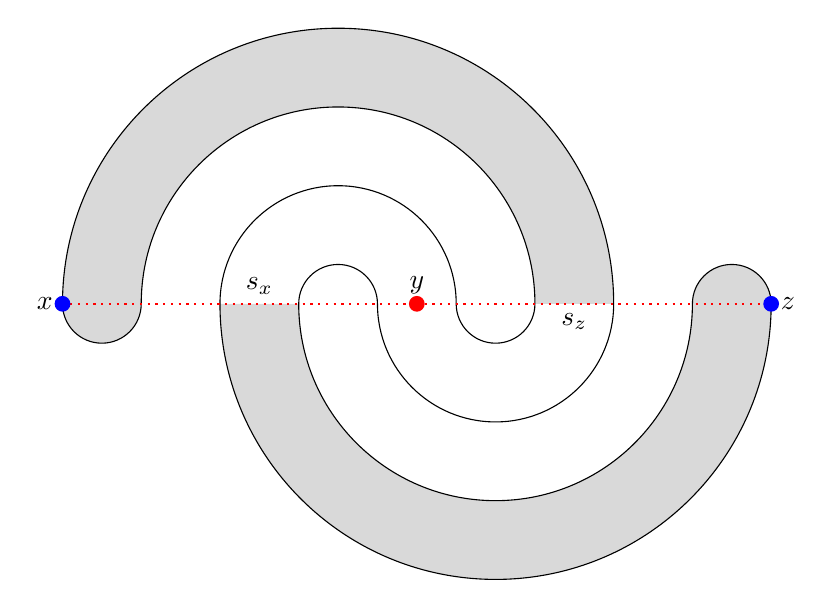
\begin{tikzpicture}

\fill[gray!30]  (7,0) arc[start angle=0, end angle=180, x radius=3.5, y radius =3.5] arc[start angle=180, end angle=360, x radius=.5, y radius =.5] arc[start angle=180, end angle=0, x radius=2.5, y radius =2.5] -- cycle;
\fill[gray!30]  (2,0) arc[start angle=180, end angle=360, x radius=3.5, y radius =3.5] arc[start angle=0, end angle=180, x radius=.5, y radius =.5] arc[start angle=0, end angle=-180, x radius=2.5, y radius =2.5] -- cycle;
\node[left] () at (0,0) {$x$};
\node[above] () at (2.5,0) {$s_x$};
\node[below] () at (6.5,0) {$s_z$};
\node[right] () at (9,0) {$z$};
\node[above] () at (4.5,0) {$y$};
\draw (7,0) arc[start angle=0, end angle=180, x radius=3.5, y radius =3.5] ;
\draw (1,0) arc[start angle=0, end angle=-180, x radius=.5, y radius =.5] ;
\draw (6,0) arc[start angle=0, end angle=180, x radius=2.5, y radius =2.5] ;
\draw (4,0) arc[start angle=0, end angle=180, x radius=.5, y radius =.5] ;
\draw (9,0) arc[start angle=0, end angle=180, x radius=.5, y radius =.5] ;
\draw (5,0) arc[start angle=0, end angle=180, x radius=1.5, y radius =1.5] ;
\draw (9,0) arc[start angle=0, end angle=-180, x radius=3.5, y radius =3.5] ;
\draw (8,0) arc[start angle=0, end angle=-180, x radius=2.5, y radius =2.5] ;
\draw (7,0) arc[start angle=0, end angle=-180, x radius=1.5, y radius =1.5] ;
\draw (6,0) arc[start angle=0, end angle=-180, x radius=.5, y radius =.5] ;
\draw[dotted, thick, red] (0,0) -- (4.5,0);
\draw[dotted, thick, red] (4.5,0) -- (9,0);
\fill[red] (4.5,0) circle(.1);
\fill[blue] (0,0) circle(.1);
\fill[blue] (9,0) circle(.1);


\end{tikzpicture}
\end{document}
